\chapter{Using Kepler’s Laws to find the density of Jupiter}

%todo include caution about rotation of image compared to website
%todo give the density of water, to aid analysis of planet as rocky or gaseous

\section{Introduction}

So far, you have been using several techniques to learn about the properties of planets orbiting other stars based one what we can observe from Earth, including using orbital properties to discover the mass of planets. The same physical laws can be used to study planets and their moons.

To study the composition of a planet, it is useful to know its density --- then one can learn more about whether it is rocky or gaseous. In this lab, you will use Kepler's Laws to find the density of Jupiter, given orbital properties of its moons. In this case, we can use actual images of the these using Stone Edge Observatory, a remotely operated telescope in California.

Under nominal circumstances, we would have you schedule the observations yourself, so you could analyze the data that you, yourself, took. However, the observatory is not operating well enough right now to let that happen. Fortunately, we have archival images that were taken in 2017 by this observatory that you can analyze.

\section{Team roles}

\begin{steps}
	\item \textbf{Decide on roles} for each group member.
\end{steps}

The available roles are:
\begin{itemize}
	\item Facilitator: ensures time and group focus are efficiently used
	\item Scribe: ensures work is recorded
	\item Technician: oversees apparatus assembly, usage
	\item Skeptic: ensures group is questioning itself
\end{itemize}

These roles can rotate each lab, and you will report at the end of the lab report on how it went for each role. Some members will be holding more than one role. For example, you could have the skeptic double with another role. Consider taking on a role you are less comfortable with, to gain experience and more comfort in that role.

Additionally, if you are finding the lab roles more restrictive than helpful, you can decide to co-hold some or all roles, or think of them more like functions that every team needs to carry out, and then reflecting on how the team executed each function.

\section{Add members to Canvas lab report assignment group}

\begin{steps}
	\item On Canvas, navigate to the People section, then to the ``Lab 4 Groups'' tab. Find a group that is not yet used, and have each person in your group add themselves to that same lab group.
\end{steps}

This enables group grading of your lab report. Only one person will submit the group report, and all members of the group will receive the grade and have access to view the graded assignment.

\section{Using Kepler's laws}

Keplers third law relates the orbital period to the systems semi-major axis. In the case where the planets mass is much smaller than the stars mass, Kepler's third law is:
\begin{equation}
P^2 = \frac{4\pi^2}{G M}a^3 \,,
\end{equation}
where $P$ is the orbital period, $G$ is Newton's constant ($6.674 \times 10^{-11}\:\textrm{N}\:\textrm{m}^2/\textrm{kg}^2$), $M$ is the mass of Jupiter, and $a$ is the semi-major axis.

We can rewrite the third law as:

\begin{equation}
\frac{a^3}{P^2} = \frac{G}{4\pi^2}\left(\frac{4}{3}\pi R^3\rho \right) = \rho\frac{G R^3}{3\pi}
\end{equation}

where $R$ is the radius of Jupiter and $\rho$ (the Greek letter pronounced ``row'') is the density of Jupiter. Solving for $\rho$ gives:

\begin{equation}\label{jd:eqn:kepden}
\rho = \left(\frac{a}{R}\right)^3\frac{3\pi}{G P^2}
\end{equation}

The goal for this lab is to use our data to determine the ratio $(a/R)$ for each moon. We can then combine that with the moons period to estimate the density of Jupiter.

To determine the semi-major axis, $a$, for a moon's orbit, we can assume that the orbit is actually a circular orbit, and we know that we are viewing the orbits edge-on. So what we are seeing is a projection of a circular motion onto one dimension, which results in a sinusoidal motion, with the amplitude of that motion being the radius of the orbit (and thus the semi-major axis). So here we will analyze images taken at different times, plot the angular position of the moon over time, fit those data points to a sine (or, equivalently, a cosine) function, and the amplitude will be the semi-major axis, $a$.

\section{The set of observations}

The images can be found on Canvas, in the Files section, in the compressed file ``jupiter\_data.zip''.

Observations were taken on four separate dates between April 14 and 23, 2017, as stated in the names of the files. Images were taken in each of the \textit{g}, \textit{r}, \textit{i}, and \textit{clear} bands. These refer approximately to the color filters used in each case: green, red, infrared, and  clear (no filter). See Figure~\ref{jd:fig:filters} for the frequency response of such a filter set. All images were taken with a $0.05\:$second exposure time.

\begin{figure}
	\centering
	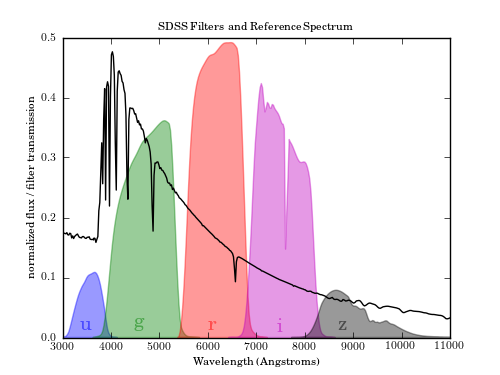
\includegraphics[width=0.8\textwidth]{jupiter-density/fig_sdss_filters_1}
	\caption{Typical transmission rates of various filters used in astronomy. This is from the Sloan Digital Sky Survey.}\label{jd:fig:filters}
\end{figure}

%\section{Make color images}
%
%All CCDs which are used in astronomical images are monochrome --- they do not have different pixels for different wavelengths of light, which allows them to achieve higher resolution. To create a color image, we must combine the images taken with different color filters and add color ourselves.
%
%One can easily make RGB images in DS9 by selecting \textit{Frame} $>$ \textit{New Frame RGB}, which allows one to upload different .fits files for each color with \textit{File} $>$ \textit{Open} depending on the color selected in the pop-up window. You can then scale each image as needed to make 3-color images. \textbf{Make an RGB image for Jupiter.}
%
\section{Analysis}

You will use the \textit{clear} images to measure the position of the moons relative to Jupiter and
\textit{gri} images to measure the radius of Jupiter. Since we will be using the ratio of moon position to Jupiter radius, we can use whatever units are convenient to measure the distance, as long as we are consistent, as the unit divides by itself in the calculation.

\begin{steps}
	
	\item Download and install DS9 from \url{http://ds9.si.edu/site/Download.html}. SAOImage DS9, or DS9 for short, is an image viewer, analyzer, and processor written and used by astronomers for working with astronomical images.
	
	If you click the link to download, it might say "redirecting" while never actually redirecting. In this case, copy the link into the address bar directly.
	\begin{framed}	
		\textbf{For MacOS}, unless you know otherwise, choose from the top set of choices (to the right of
		the blue apple logo). To find your version, from the Apple menu in the corner of the screen,
		choose “About This Mac”.
		
		If it displays a warning and prevents you from installed from an unidentified developer, follow the instructions at the following link to create an exception:
		
		\url{https://support.apple.com/guide/mac-help/open-a-mac-app-from-an-unidentified-developer-mh40616/mac}
	\end{framed}

	\item Open the Google Sheet found here: \url{https://docs.google.com/spreadsheets/d/1y1vfi3l1KzGoE0cOctwA0Z5s7ioptaRFpSLItBoRv2c/edit?usp=sharing}
	
	\item Make a copy of this sheet for your group to use. Explore the parts of the sheet. Notice the model equation and fit parameters at the top. Notice the data columns, including the time, distance from the center of Jupiter \texttt{x}, and the radius of Jupiter \texttt{R\_Jupiter}. There is also a plot of the measured and model $x/R$. There is a different sheet for each moon you are observing. Notice the different tabs at the bottom of the window for each of the four moons.
	
	\item Download the Jupiter data zip file from Canvas and extract it to a folder on your computer.
	
	\item Start DS9 and open the file from the earliest timestamp, with the clear filter.
	
	\item \textbf{Record the time} the image was taken by going to the \textit{File} menu and then \textit{Display Fits Header}. Towards the bottom of the header will be listed the \textit{DATE-OBS} which will be in the UTC timezone.
	
	\item Convert the time given to decimal time in days after 2017-04-14T00:00:00. It may help to use the converter below the plot in the spreadsheet.
\end{steps}

In the data table, there is an entry for each tenth of a day, so that the model $x/R$ can be computed and plotted.

\begin{steps}
	\item To include your measurement, insert a new row for the image's timestamp by right-clicking the row number of the time just before the image's timestamp and selecting ``Insert 1 below''.
	
	\item Enter your image's decimal time in the time column.

	\item Identify the moons in your image by doing the following:
	\begin{enumerate}
		\item Adjust the contrast and zoom in your image until you can clearly see Jupiter and four moons. To get a better view, select ``Scale $>>$ Log'' from the drop-down menus, and also right-click-drag up, down, left, and right anywhere on the image to adjust the contrast dynamically.
		
		\item In another browser tab, open \url{http://www.shallowsky.com/jupiter/}, enter the observation time, and press the circular arrow ``refresh'' symbol. It automatically adjusts for your local timezone (in Chicago it adds ``-5'' to the end of the timestamp.), so to unadjust back to UTC, do that arithmetic operation to the entered time. In the case of Chicago and ``-5'', subtract 5 hours from the entered time.
		
		\item Ensure the images match and correct the time if necessary. If the image seems flipped or rotated, select a different orientation from the drop-down.
	\end{enumerate}
	
	\item \textbf{Use} DS9 to measure the distance from the center of Jupiter to each moon using the Ruler function described in the following paragraph. Keep track of whether the moon is on the East or West side of Jupiter by making all locations on the left side positive and locations on the right side negative. \textbf{Record your value} in the data table for each moon.
\end{steps}

You can use the DS9 \textit{Ruler} function to measure the distance (in pixels) between two points in the image. To use the \textit{Ruler}, first go to the Region menu from the toolbar at the top. Select the \textit{Shape} sub-menu and click \textit{Ruler}. Then, click the \textit{Edit} menu button and select \textit{Region}. You can then use the mouse to draw a line between two points and DS9 will calculate the distance for you. If you have trouble using the \textit{Ruler} feature, you can also read off the $(x,y)$ coordinates for each point and calculate the distance yourself using Pythagorean's theorem.

\begin{steps}
	\item Repeat the above analysis for each of the four timestamps.
\end{steps}

The apparent radius of Jupiter can be different for each image, since the apparent brightness can change depending on local weather conditions. So if available, you will measure its radius for each timestamp.

\begin{steps} 
	\item For each timestamp, if its available, load the image taken with the ``i'' filter, listed in the filename, and measure Jupiter's radius, recording it in the table. If there is no such image, take an average of the other image's measured radii.
\end{steps}

You should now have 4 distances for each of the four moons recorded in their respective data tables. Now you will plot them and fit the sine functions, to find the semi-major axis of each one.

\section{Plotting and fitting}

\begin{steps}
	\item For each row of measured data, enter the formula for the ``$x/R$ measured'' row. In Google Sheets, the procedure is as follows:
	\begin{enumerate}
		\item Select the cell in which you want to enter the formula (to the right of your measured \texttt{R\_Jupiter}.)
		
		\item Enter ``\texttt{=}'', click the cell that contains your measured $x$ to insert that cell's identifier, enter ``/'', click the cell that contains your measured $R_J$, and press enter. Ensure that it divided the correct values.
	\end{enumerate}

	\item In the next column, marked ``x/R model'', you need to continue the formula from the row above, in order to computer the model x/R for that timestamp. To do this, click on the cell in the row above, then click and drag the box on the lower right of the cell's border down by one cell.
	
	\item Do the same for the \texttt{diff\^{}2} column.
\end{steps}

Now you should have all four data points displaying on the plot, for each moon, and you are ready to fit the sine curve for each moon, so you can find the ratio semi-major axis divided by Jupiter radius, $a/R$, as needed for applying Kepler's third law as in Equation\ \ref{jd:eqn:kepden}.

\begin{steps}
	\item For each moon, enter the period of its orbit (from Table\ \ref{jd:tab:periods}) in the fit parameter for period, \texttt{B}.
	
	\item For each moon, adjust the other fit parameters, amplitude and time offset, to visually match the measured points, and then fine-adjust to minimize the rms deviation.
\end{steps}

\begin{table}
	\centering
	\begin{tabular}{ l c r }
		\hline
		Moon & Period (days) & $\rho_\textrm{Jupiter}$ $(\textrm{kg/m}^3)$\\
		\hline
		Ganymede & 7.1546 & \\
		Io & 1.7691 & \\
		Europa & 3.5512 & \\
		Calisto & 16.689 & \\
		\hline  
	\end{tabular}
	\caption{Four moons of Jupiter and their periods.}\label{jd:tab:periods}
\end{table}

The amplitude from your fit corresponds to the ratio, $(a/R)$ which we will use in Kepler’s Third law.

\begin{steps}
	\item For each moon, use the amplitude of the curve together with Kepler's Third law
	to estimate the density of Jupiter. Make sure you use the right units for your values. \textit{Hint:
	look at the units for the Gravitational constant. What units do you need for the moons
	orbital period?}

	\item\label{jd:step:density} Take the average of the densities, and use the standard deviation of them for the uncertainty. Report this value, with uncertainty, in your report.
	
	\item Compare your result to a value of the density you find online, using the uncertainties and the procedure in Appendix~\ref{unc:sec:comparing}. How close are they? What are possible sources of uncertainty of your measurement?
	
	\item\label{jd:step:composition} Rocky planets in our solar system have densities ranging from 3000--5000$\:$kg/m$^3$, and water has a density of 1000$\:$kg/m$^3$ (atmospheric air at sea level on Earth has a density of about 1$\:$kg/m$^3$). Given these ranges and your result, would you conclude that Jupiter is rocky or gaseous, and why?
\end{steps}

\section{Report checklist and grading}

Each item below is worth 10 points, and there is an additional 10 points for attendance and participation.

\begin{enumerate}
	\item Data table including times and positions for each moon, as well as the radius of Jupiter.
	
	\item Graphs of position ($x/R$) vs. time for each moon, with the fitted curve plotted as well.
	
	\item Answers or evidence of completion for Steps~\ref{jd:step:density}--\ref{jd:step:composition}.
	
	\item A 100--200 word reflection on group dynamics and feedback on the lab manual. Address the following topics: who did what in the lab, how did you work together, what successes and challenges in group functioning did you have, and what would you keep and change about the lab write-up?
	
\end{enumerate}